\documentclass[a4paper,12pt,twoside]{article}
\usepackage[inner=3cm,outer=2.5cm,top=2.5cm, bottom=2.5cm]{geometry} %left=4cm,right=2cm would be equivalent
\usepackage[utf8]{inputenc}
\usepackage{t1enc}
\usepackage{graphicx}
\usepackage[magyar]{babel}
\usepackage[nottoc]{tocbibind}%hogy az irodalomjegyzék is benne legyen a tartalomjegyzékben

\usepackage{commath} %abszolút érték jelhez.
\usepackage{multirow}
\usepackage{subcaption}
\usepackage{subfig}
%matgót megoldottam a 2. sorban.
%\usepackage{anysize} %margóhoz
%\marginsize{3cm}{3cm}{2.5cm}{2.5cm}


%ha esetleg ki akarod szerni az összes ábrát ->
%\usepackage{comment}
%\excludecomment{textcolor}
%\excludecomment{figure}
%\let\endfigure\relax
%<-
\linespread{1.3} %1.3 = másfélszeres sorköz.
%\usepackage{showframe} -> megjelnnek a margók.

\begin{document}
\frenchspacing
%%%%%%%%%%%%%%%%%%%%%%%%%%%%%%%%%%%%%%%%%%%%%%%%%%%%%%%%%%%%%%%%%


\pagenumbering{gobble}

 \begin{center} \includegraphics[width=80mm,keepaspectratio]{abrak/bmelogo.jpg}\\ \vspace{0.3cm}  \Large Diplomamunka \\[1.5cm] \vspace{0.5cm} { \large \textbf{ Cím}}\\[2.5cm] \vspace{0.2cm} \large Marinovszki Árpád\\[5cm] \begin{tabular}{ll} Témavezető: & Dr.\ Légrády Dávid \\ & egyetemi docens \\ & BME Nukleáris technika Intézet \\ \end{tabular} \vfill \large BME \\ \large 2016 \end{center} 
 
 \clearpage \setcounter{page}{1}
 \pagenumbering{arabic}
 


{\large A szakdolgozat kiírása}




\begin{tabular}{ll}
\multicolumn{2}{c} {Témavezető:} \\
Neve:&Légrády Dávid\\
Tanszéke:&NTI\\
E-mail címe:&legrady@reak.bme.hu\\
Telefonszáma:&1254 \\
\end{tabular}

\begin{tabular}{||p{0.25\textwidth}||p{0.64\textwidth}||}
\hline
\hline
\multicolumn{2}{||l||}{Azonosító: Azomosító}\\
\hline
\hline
Szakdolgozat címe:&G Cím\\
\hline
\hline
Melyik szakiránynak ajánlott?&,Szakirány\\
\hline
\hline
A jelentkezővel szemben támasztott elvárások:& Elvárások\\
\hline
\hline
Leírása:&Leírás \\
\hline
\hline \end{tabular}

\clearpage

{\large Önállósági nyilatkozat}
\\[0.5cm]


Nyilatkozat.\\[0.3cm]


Budapest, 2016.\ június 6.

\hspace{9cm}\makebox[1.5in]{\hrulefill}

\hspace{9cm}\makebox[1.5in]{\centering aláírás}




\clearpage


 \tableofcontents

\clearpage

	






%CSAPJUNK A LECSÓBA
%TODO majd egyeztesd az egyes fejezeteken belül a személyeket és az igeidőt (csináljuk / csinálják/ csinálták stb)
%BEVEZETÉS------------------------------------------------------
\section{Bevezetés}

\section{Gain korrekció}


A gain korrekció az elkészült felvételeken elsődlegesen elvégzendő korrekció, amely felelős egyrészt azért, hogy a detektorpixelek eltérő érzékenysége és zaja következtében fellépő képhibákat eltüntesse. Továbbá, hogy korrigálja a röntgennyaláb mért intenzitásában történő azon gyengülést, amely pusztán azért következik be, mert a detektorpixelek más--más távolságra vannak a forrástól.

A fejezet elején megmutatom, hogy milyen hibákat eredményez a gain korrekció elhanyagolása. Ez után ismertetem a korrekció elvégzéséhez szükséges algoritmusokat, majd bemutatom, hogy implementáltam ezeket az elkészült programban. 

\subsection{A gain korrekció által javított artefaktumok bemutatása}

A gain korrekció által kiszűrt hibák három részre oszthatóak. Egyrészt belátható, hogy a sík detektoron mérhető fluxus értéke nem egyenletes. Ha olyan felvételt tekintünk, ahol nincs leképezendő objektum, belátható, hogy a legnagyobb fluxus a detektor azon pixelét fogja érni, amely a legközelebb van a röntgenforrás fókuszpontjához. Az ettől távolabbi pixeleken mérhető intenzitás pusztán azért is kisebb lesz, mert a forrásponttól távolabb vannak, hiszen a mérhető intenzitás a fókuszponttól számított távolság négyzetének inverzével arányos. A jelenség következtében tehát a detektorpixelek intenzitása a szélek felé csökken, és a csökkenés mértéke az expozíciós beállításoktól -- úgy mint az expozíciós idő, valamint a röntgencső feszültsége és árama -- független. A kialakult képtorzulást \emph{flatness hibának} nevezzük.

Megállapítható továbbá, hogy a detektorpixelek eltérő érzékenysége miatt is fellépnek képhibák. Ezen hibákat két csoportra lehet bontani: \emph{offset hibára}, valamint \emph{gain hibára}. Az elnevezés igen szemléletes. Válasszunk ki a detektoron egy adott pixelt, és vizsgáljuk ennek a pixelnek az mért intenzitását, miközben változtatjuk az expozíciós időt! Az adott pixelen a mért intenzitás -- expozíciós idő függvényt ábrázolva olyan görbét kapunk, amely kezdetben igen jó közelítéssel egyenest mutat, mígnem az intenzitás egy adott értéket elérve nem nő tovább. Utóbbi esetet, azaz, amikor az intenzitásérték tovább nem nő, szaturációnak hívjuk. Az előbbihez hasonlóan, ha állandó expozíciós idő mellett a röntgencső áramerősségét változtatjuk, és így nem a felvétel idejét növeljük, hanem a detektorra eső nyalábintenzitást, szintén kezdetben lineáris, majd telítődő összefüggést kapunk a pixel által mért intenzitás -- alkalmazott áramerősség függvény tekintetében. Éppen ezért az expozíciós idő és a röntgencső áramerősségének szorzatának -- a továbbiakban \emph{expozíció} függvényében szokás vizsgálni az adott pixel intenzitását. Az így kapott görbe, azaz az intenzitás az expozíció függvényében, adja meg az adott pixel érzékenységét.

Az érzékenység azonban pixelről pixelre változik. Különböző pixelek érzékenységét megvizsgálva észrevehetjük, hogy az egyes érzékenységi görbék lineáris szakaszának meredeksége és tengelymetszete is változik. Változik továbbá a szaturációs expozíció is, azaz az az expozíció érték, amelynél az adott detektor telítésbe megy. Ezt szemlélteti \aref{fig:gaingrafikon}.~ábra, amelyen négy különböző pixel által mért intenzitást ábrázoltam, az expozíció függvényében. Az ábrán jól látszódik, hogy a különböző pixelek érzékenysége eltérő meredekségű és tengelymetszetű egyenessel jellemezhető, valamint a szaturációs expozíciójuk is eltérő. Az offset és gain korrekciók a detektorpixelek ezen érzékenységbeli különbségeit korrigálják. Az \emph{offset hibák} javítása jelenti a lineáris szakaszok eltérő tengelymetszetőből származó eltérések kiküszöbölését. Az offset  hibák nagysága nem függ tehát az expozíciótól, de függ az expozíciós időtől. Ugyanis kikapcsolt röntgenforrás mellett is detektálunk valamekkora háttérsugárzást, illetve a detektorok zaja is mérhető intenzitást fog eredményezni a felvételen. A teljes, röntgenforrás nélkül mért jel tehát arányos lesz az expozíciós idővel.  A \emph{gain hibák} javítása jelenti az érzékenységek lineáris szakaszainak eltérő meredekségéből, valamint az eltérő szaturációs expozíciókból származó hibák javítását. Ezek tehát az expozíciós beállításoktól függő hibák.





\begin{figure}[htbp]
\center
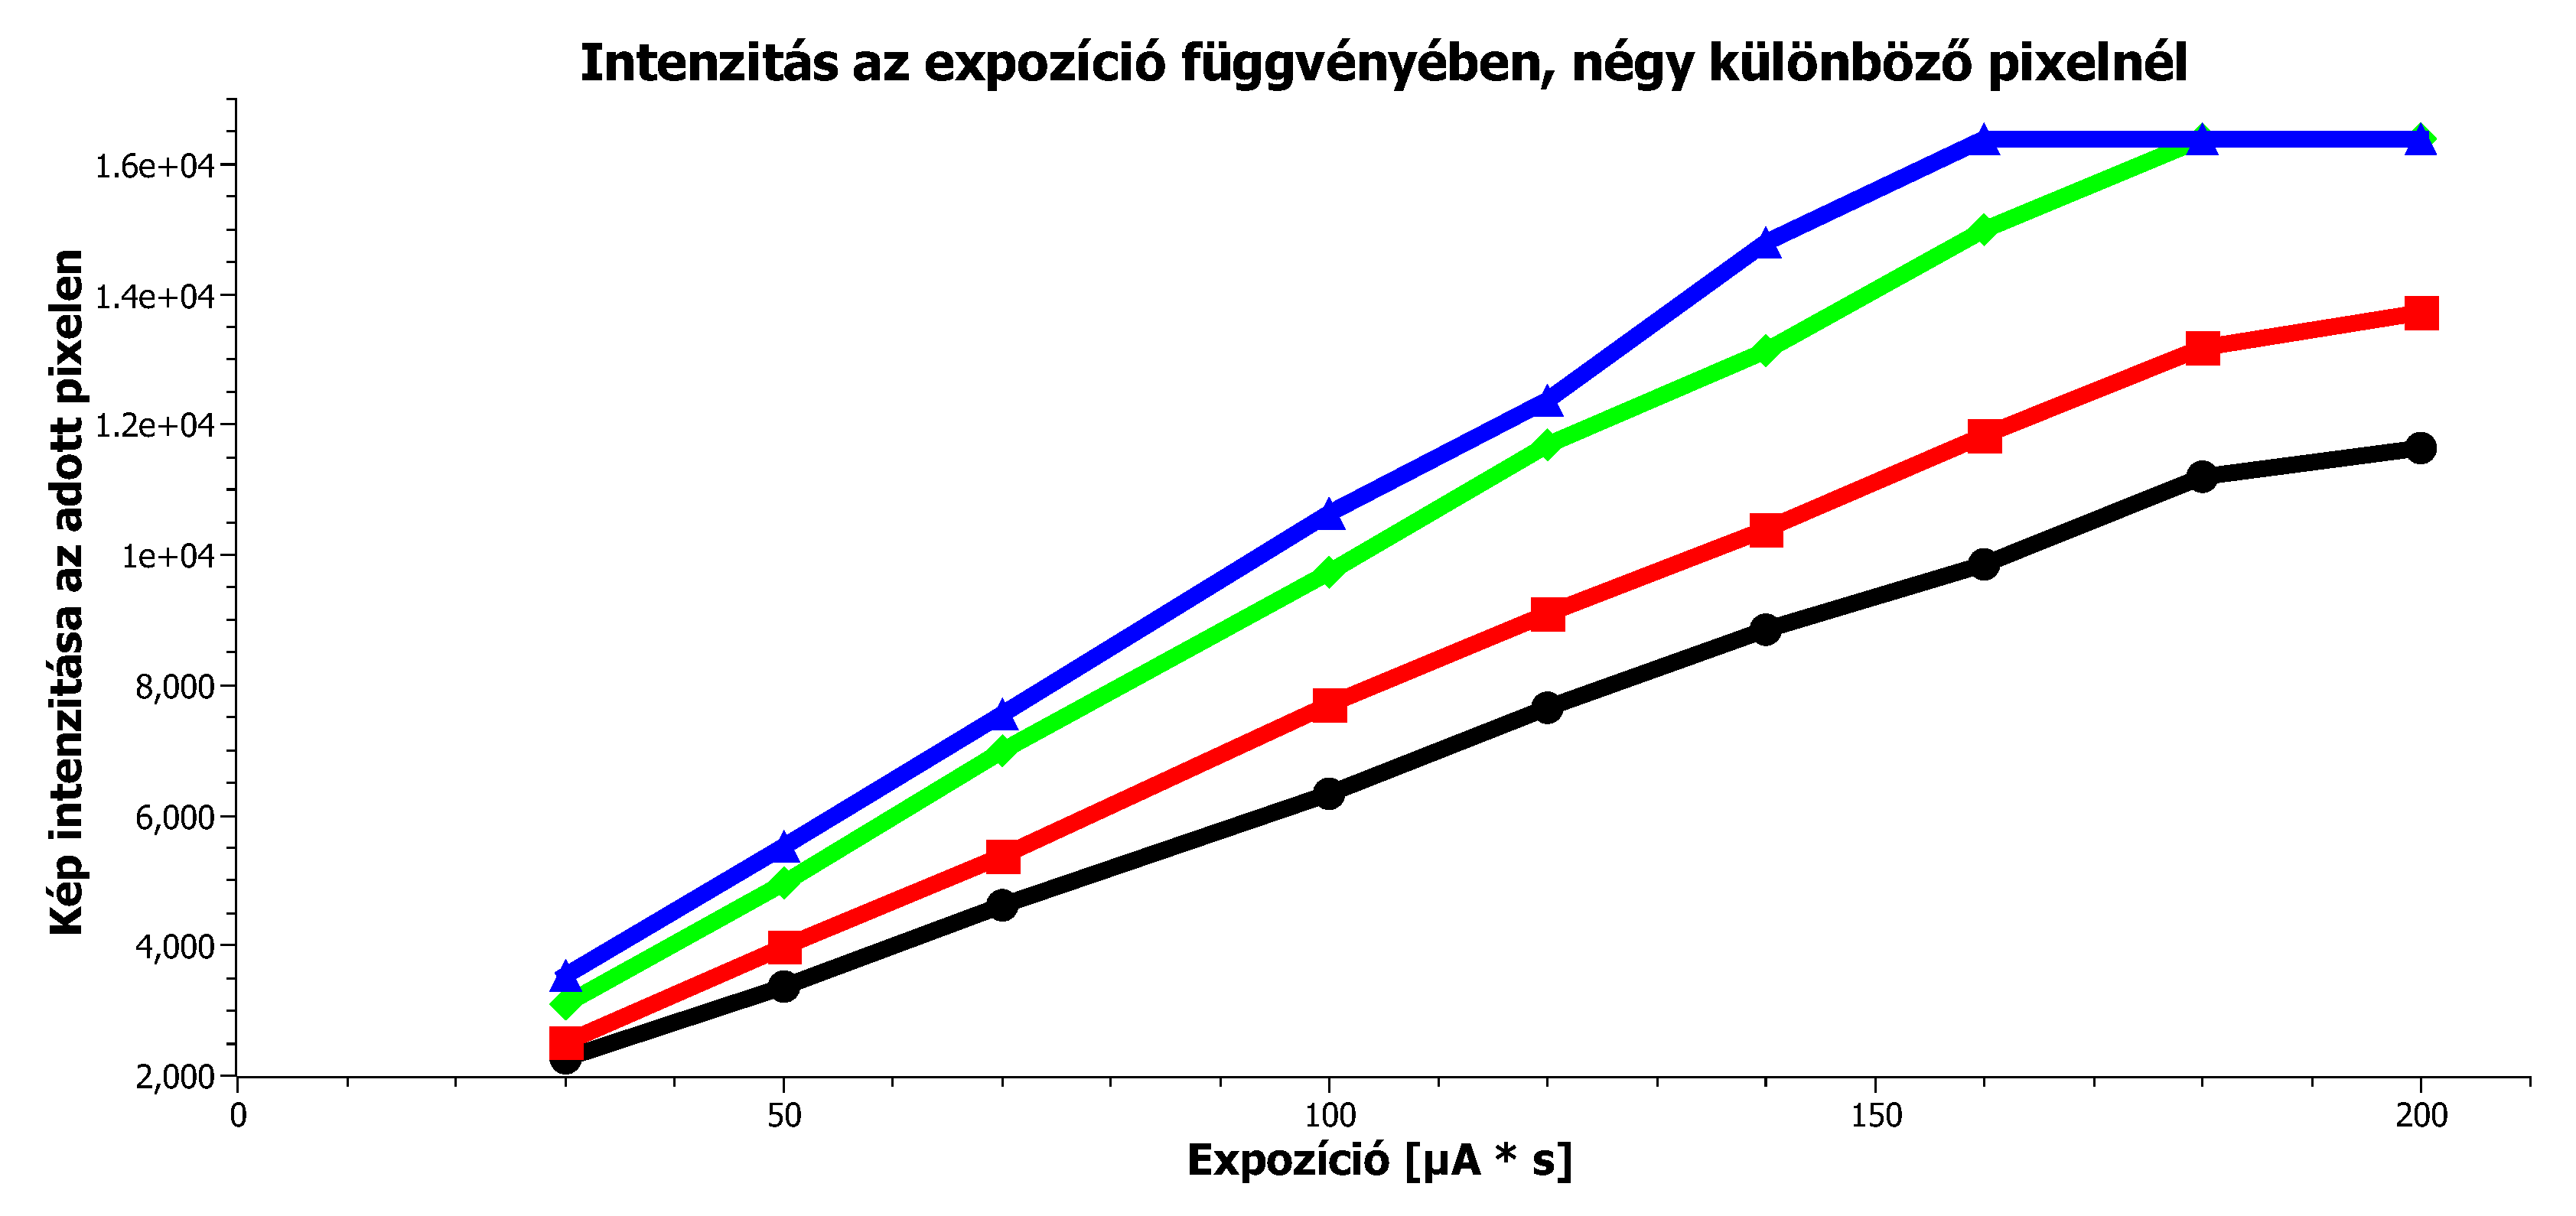
\includegraphics[width=0.8\textwidth]{abrak/gaingrafikon}
\caption{Négy kiszemelt pixel intenzitásának változása az expozíció függvényében.}
\label{fig:gaingrafikon}
\end{figure}



A felvételek készítésekor rögtön szembetűnik ugyanis, hogy a kapott kép a homogénnek várt területeken sem teljesen homogén, illetve a detektorpanel struktúlátsága artefaktumokok, azaz képhibák megjelenését okozza a felvételen. Ezt szemlélteti \aref{fig:gainnelkul}.~ábrán látható felvétel, amely egy gain korrigálás nélküli felvétel. A felvétel készítésekor a röntgensugár útjába nem helyeztünk tárgyat.

Egy ilyen felvételtől azt várjuk, hogy ,,fehér'' képet adjon, avagy a képen a pixelek intenzitása mindenhol megegyezzen, és lehetőleg a röntgencső beállításától függetlenül mind maximumot adjon -- hiszen nincs leképezendő objektum a forrás és a detektor között. Az ábrán azonban szembetűnően látszik, hogy az első elvárásunk, amely szerint a kép homogén legyen, messze nem teljesül. A továbbiakban bemutatom az röntgencső adott beállításai mellett készült felvétel hibáit. Ez után pedig kitérek a második kritériumnak való megfeleltetés kérdésére, azaz hogy a különböző expozíciós beállításokkal készült felvételek 

\begin{figure}[htbp]
\center
\includegraphics[width=0.8\textwidth]{abrak/gainnelkul}
\caption{Tárgy nélkül készített felvétel, gain korrigálás nélkül.}
\label{fig:gainnelkul}
\end{figure}


\clearpage

\begin{thebibliography}{9}


%\bibitem{url}
%{\tt http://fizipedia.bme.hu/index.php/Gamma\_spektroszkópia},
%2013.~november~29., 1:00

%\bibitem {nagy}
%Nagy L. Gy.,
%{\it Radiokémia és izotóptechnika},
%Tankönyvkiadó, Budapest, 1983.
%\bibitem {lederer}
%C.M. Lederer, J.M. Hollander, I. Perlman,
%{\it \foreignlanguage{english}{Table of Isotopes}},
%Wiley, New York, 1984.
\end{thebibliography}
\end{document}